
%----------------------------------------------------------------------------------------
%	PACKAGES AND THEMES
%----------------------------------------------------------------------------------------

\documentclass[aspectratio=169]{beamer}
\mode<presentation> {
	
	\usetheme{Boadilla}
}
\usepackage{xcolor}
\definecolor{lmugreen}{RGB}{0, 136, 58}
\usecolortheme[named=lmugreen]{structure}
\definecolor{pastelBlue}{RGB}{102,153,204}   % soft blue
\definecolor{pastelRed}{RGB}{204,102,102}    % soft red
\usepackage{graphicx} % Allows including images
\usepackage{booktabs} % Allows the use of \toprule, \midrule and \bottomrule in tables
\usepackage[english]{babel}
\usepackage[utf8]{inputenc}
\usepackage{amsmath,amssymb} % math symbols
\usepackage{graphicx}
\usepackage{float}
\usepackage{hyperref} % for URLs
\newcommand{\gray}{\rowcolor[gray]{.90}}
\usepackage{verbatim}
\usepackage{textpos} % logo position
\usepackage[default]{sourcesanspro} % font type
\usepackage{cases} % math cases
\usepackage{tikz}
\usetikzlibrary{arrows.meta, positioning, shapes}
% Put this in your preamble:

% Caption
\usepackage{caption}
\DeclareCaptionFont{tiny}{\tiny}
\captionsetup{font=scriptsize,labelfont=scriptsize,justification=centering}

% ToC
\AtBeginSection[]{
	\begin{frame}[noframenumbering, plain]
	\frametitle{Outline}
	\setcounter{tocdepth}{1}
	\tableofcontents[currentsection]
\end{frame}
}

% Remove navigation 
\beamertemplatenavigationsymbolsempty

% R 
\usepackage{listings}
\lstset{
language=R,
basicstyle=\scriptsize\ttfamily,
commentstyle=\ttfamily\color{gray},
backgroundcolor=\color{white},
showspaces=false,
showstringspaces=false,
showtabs=false,
tabsize=2,
captionpos=b,
breaklines=false,
breakatwhitespace=false,
title=\lstname,
escapeinside={},
keywordstyle={},
morekeywords={}, 
belowskip = -1.2 \baselineskip,
}

%----------------------------------------------------------------------------------------
%	TITLE PAGE
%----------------------------------------------------------------------------------------

\addtobeamertemplate{frametitle}{}{%
	\begin{textblock*}{100mm}(0.88\textwidth,-0.5cm)
		
\includegraphics[height=1cm,width=2cm]{lmu_logo}
\end{textblock*}}

%
\includegraphics[width=0.3\textwidth]{lmu_logo}
\vspace*{-1cm}

\title{Functional ANOVA Decomposition} 

\author{Juliet Fleischer} 
\institute[LMU]{LMU} % Your institution as it will appear on the bottom of every slide, may be shorthand to save space
{

}
\begin{document}

{
\usebackgroundtemplate{
\includegraphics[width=\paperwidth]{lmu-background.pdf}}
\begin{frame}
\begin{columns}
	\begin{column}{0.4\textwidth}
		\vspace{3cm}
		
		\textbf{\textcolor{white}{Functional ANOVA Decomposition}}\\
		\vspace{1cm}

		\textcolor{white}{\footnotesize Juliet Fleischer \\
			\today}
	\end{column}
	\begin{column}{0.49\textwidth}
		\vspace{2cm}
		\begin{center}
			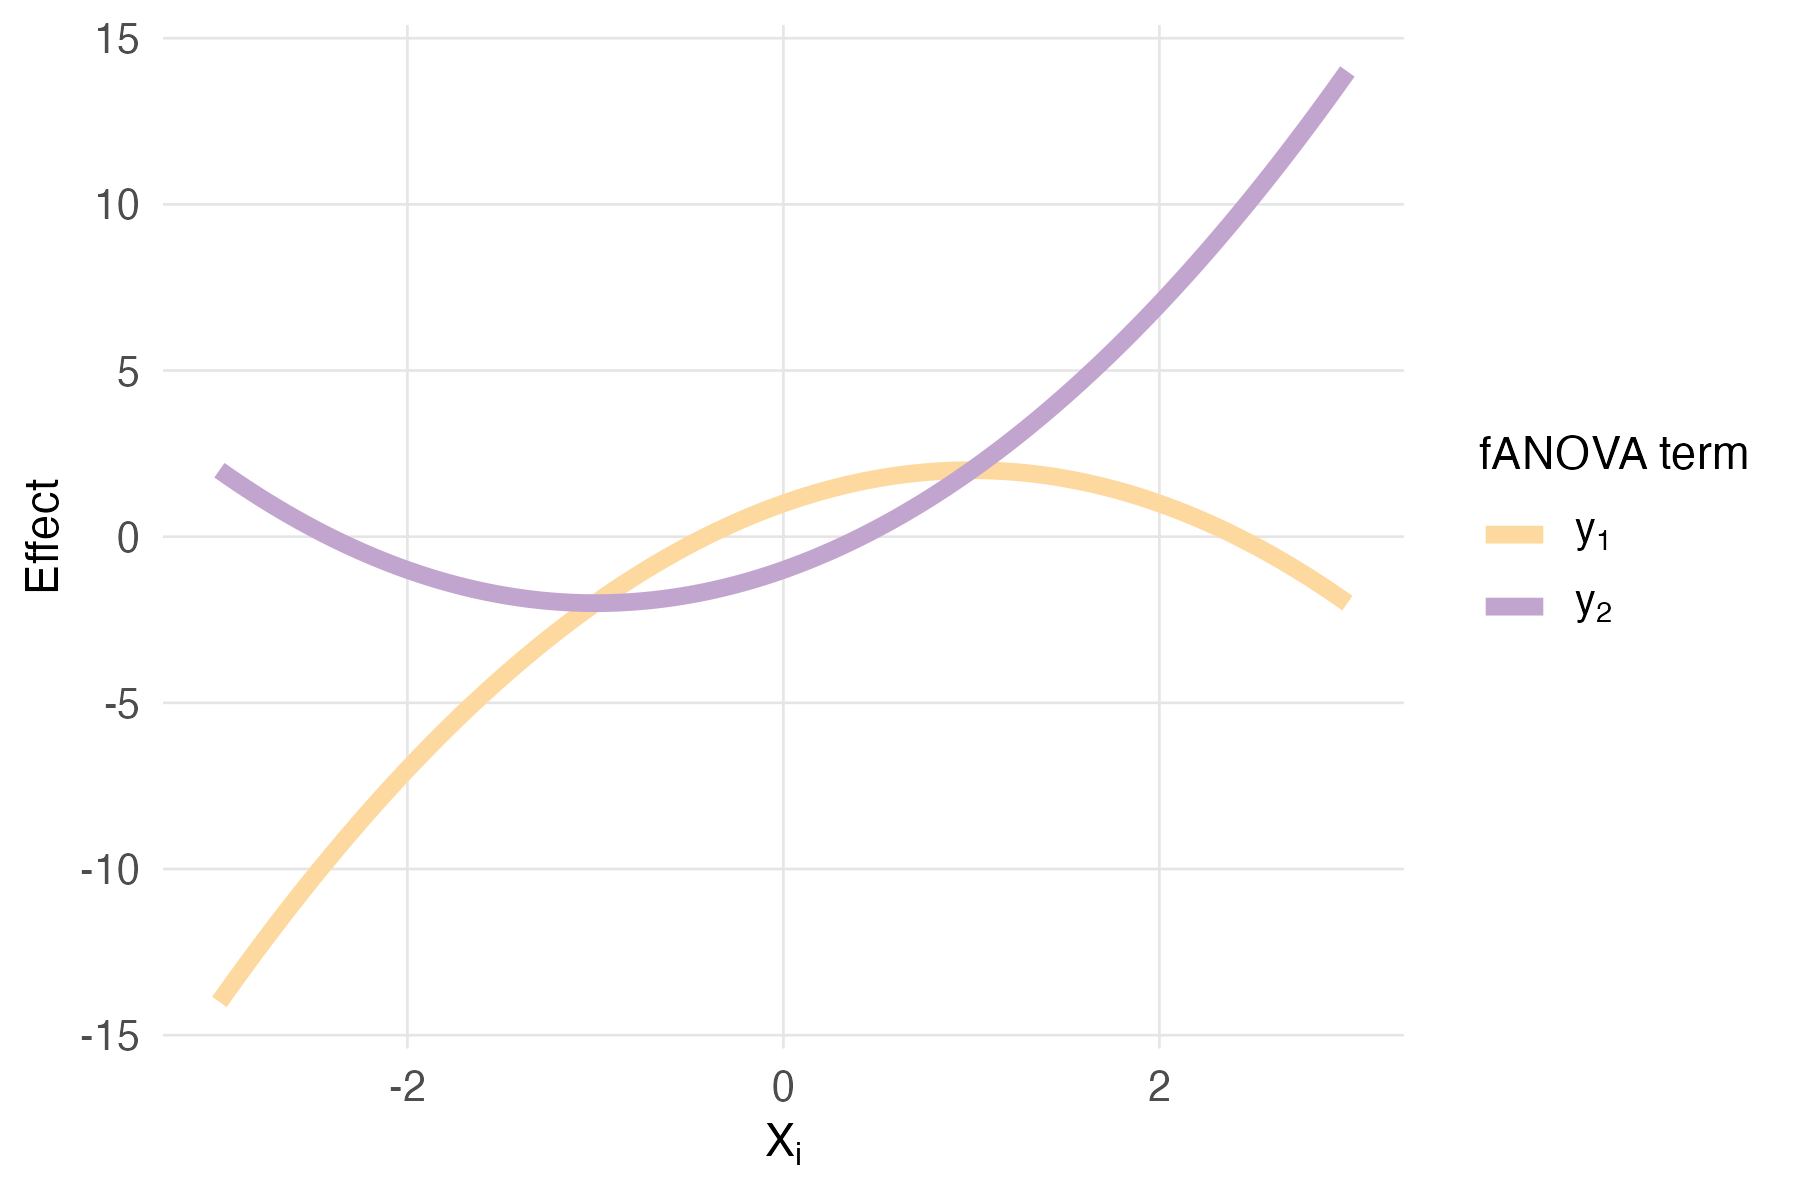
\includegraphics[width=1\textwidth]{../images/experiment_section/mixed_a1p20_a2p20_a11m10_a22p10_a12p00_rhop00_main.png}
		\end{center}
	\end{column}
\end{columns}
\end{frame}
}
%----------------------------------------------------------------------------------------
%	PRESENTATION SLIDES
%----------------------------------------------------------------------------------------


\section{Research Context}

\begin{frame}{Overview of the fANOVA Research Field}
\centering
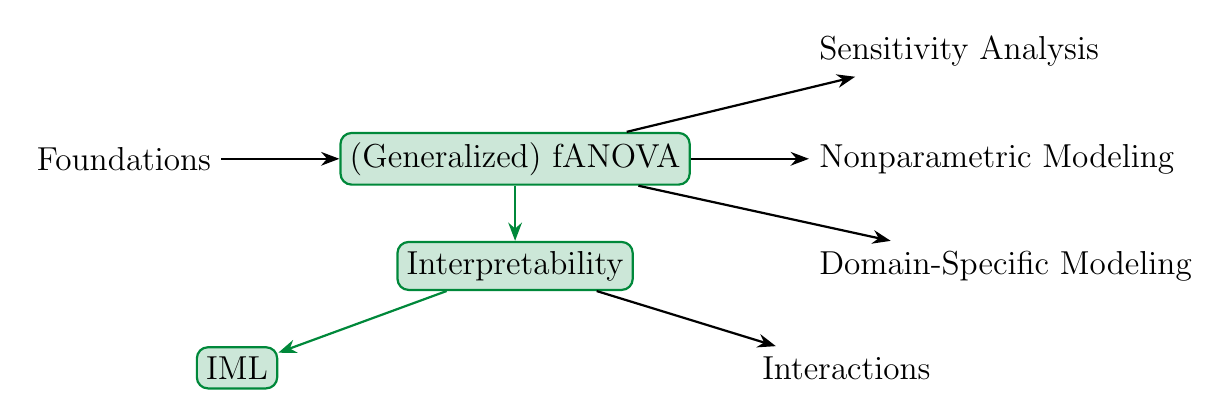
\begin{tikzpicture}[
    node distance=0.7cm and 1.5cm,
    every node/.style={font=\large},
    >=Stealth, thick
]

% Nodes
\node (foundations) {Foundations};
\node[right=of foundations, draw=lmugreen, fill=lmugreen!20, rounded corners] (fanova) {(Generalized) fANOVA};
\node[above right=of fanova] (sensitivity) {Sensitivity Analysis};
\node[right=of fanova] (nonparam) {Nonparametric Modeling};
\node[below right=of fanova] (domain) {Domain-Specific Modeling};
\node[below=of fanova, draw=lmugreen, fill=lmugreen!20, rounded corners] (interpret) {Interpretability};
\node[below left=of interpret, draw=lmugreen, fill=lmugreen!20, rounded corners] (iml) {IML};
\node[below right=of interpret] (interactions) {Interactions};

% Arrows
\draw[->] (foundations) -- (fanova);
\draw[->] (fanova) -- (sensitivity);
\draw[->] (fanova) -- (nonparam);
\draw[->] (fanova) -- (domain);
\draw[->, color = lmugreen] (fanova) -- (interpret);
\draw[->, color = lmugreen] (interpret) -- (iml);
\draw[->] (interpret) -- (interactions);

\end{tikzpicture}

\vspace{0.5cm}
\footnotesize
References: \cite{hooker2004,hooker2007,rahman2014,stone1994,sobol1993sensitivity,lengerich2020,konig2024}

\end{frame}





\section{Classical fANOVA}
\begin{frame}{Formal Setting}
  \begin{itemize}
    \item measure space, probability measure, random vector, subvector, complementary vector, pdf
    \item measure space of square integrable functions
    \item inner product
    \item norm
  \end{itemize}
  
\end{frame}

\begin{frame}{Decompose model into interpretable components} % What is it?
\begin{block}{General Form}
\[
  \begin{aligned}
    y(\boldsymbol{X}) 
    &= \sum_{u \subseteq \{1,\dots,N\}} y_{u}(\boldsymbol{X}_u) \\[3pt]
    &= y_{\emptyset} 
       + \big( y_{\{1\}}(\boldsymbol{X}_1) + \dots + y_{\{N\}}(\boldsymbol{X}_N) \big) \\[2pt]
    &\quad + \big( y_{\{1, 2\}}(\boldsymbol{X}_1,\boldsymbol{X}_2) 
                 + y_{\{1, 3\}}(\boldsymbol{X}_1,\boldsymbol{X}_3) + \dots \big) \\[2pt]
    &\quad + \big( y_{\{1, 2, 3\}}(\boldsymbol{X}_1,\boldsymbol{X}_2,\boldsymbol{X}_3) + \dots \big) 
       + \dots + y_{\{1, \dots, N\}}(\boldsymbol{X}_1, \dots, \boldsymbol{X}_N)
  \end{aligned}
\]
\end{block}

  \begin{itemize}
    \item $y$ : Model
    \item $y_u$ : Component functions for subset $u$
    \item Assumption: $X_1, \dots, X_N$ are independent
  \end{itemize}
\end{frame}

\begin{frame}{Ensure Uniqueness and Interpretability of the Components} % What conditions do we need?
  \begin{block}{Strong Annihilating Conditions}
    \[
      \int_{\mathbb{R}} y_u(\boldsymbol{x}_u) f_{\{i\}}(x_i) \, d\nu(x_i) = 0 \quad \text{for} \ i \in u \neq \emptyset.
    \]
  \end{block}
  \begin{itemize}
    \item Ensures unique component functions
    \item Applies under independent (product-type) input distributions
  \end{itemize}
    \[
    \mathbb{E}[y_u(\boldsymbol{X}_u)] = 0
  \]
  \[
    \mathbb{E}[y_u(\boldsymbol{X}_u) y_v(\boldsymbol{X}_v)] = 0 \quad (u \neq v)
  \]
\end{frame}


\begin{frame}{Recursive Form of the Components} % How do we construct it?
    \[
    y_{\emptyset} = \int_{\mathbb{R}^N} y(\boldsymbol{x}) \prod_{i=1}^{N} f_{\{i\}}(x_i) \, d\nu (x_i) = \mathbb{E}[y(\boldsymbol{X})].
    \]
\begin{equation}
    y_u(\boldsymbol{X}_u) 
    = \int_{\mathbb{R}^{N- |u|}} 
        y(\boldsymbol{X}_u, \boldsymbol{x}_{-u}) 
        \prod_{i=1, i \notin u}^{N} f_{\{i\}}(x_i) 
        \, d\nu (x_i) 
      - \sum_{v \subsetneq u} y_v(\boldsymbol{X}_v).
    \label{eq:fanova_components_classical}
\end{equation}
  \begin{itemize}
    \item $f_{-u}$ : marginal density of variables not in $u$
    \item Components solved sequentially by increasing order
  \end{itemize}
\end{frame}

\begin{frame}{Recursive Form Example}
  \begin{itemize}
    \item $N = 3$
  \end{itemize}
    \[
    y_{\emptyset} = \int_{\mathbb{R}^3} y(\boldsymbol{x}) \prod_{i=1}^{3} f_{\{i\}}(x_i) \, d\nu (x_i) = \mathbb{E}[y(\boldsymbol{X})].
    \]
  \begin{itemize}
    \item $u = \{1\}$ $\rightarrow$ $v = \emptyset$
  \end{itemize}
    \begin{equation*}
    y_{\{1\}}(X_1) 
    = \int_{\mathbb{R}^{2}} 
        y(X_{1}, x_{2}, x_{3}) 
        \prod_{i=2}^{3} f_{\{i\}}(x_i) 
        \, d\nu (x_i) 
      -  y_{\emptyset} = \mathbb{E}[y(X_1, X_2, X_3)|X_1 = x_1] - y_{\emptyset}.
\end{equation*}
  \begin{itemize}
    \item $u = \{1,2\}$ $\rightarrow$ $v = \{1\}, \{2\}, \emptyset$
  \end{itemize}
    \begin{align*}
    y_{\{1,2\}}(X_1, X_2) 
    &= \int_{\mathbb{R}} 
        y(X_1, X_2, x_3) 
        f_{\{3\}}(x_3) 
        \, d\nu (x_3) 
      -  y_{\{1\}}(X_1) -  y_{\{2\}}(X_2) - y_{\emptyset} \\
    &= \mathbb{E}[y(X_1, X_2, X_3)|X_1 = x_1, X_2 = x_2] - y_{\{1\}}(X_1) - y_{\{2\}}(X_2) - y_{\emptyset}.
\end{align*}
  
\end{frame}


\begin{frame}{Example: Independent MVN} % Example of a 2D function
  \begin{align*}
    y(x_1, x_2) = 2x_1 + x_2^{2} + x_1 x_2
  \end{align*}
\[
(X_1, X_2)^\mathsf{T} \sim \mathcal{N}\!\left(
\begin{pmatrix}0 \\ 0\end{pmatrix},
\begin{pmatrix}
1 & \rho \\ 
\rho & 1
\end{pmatrix}
\right),
\]
\[
X_1 \mid X_2=x_2 \sim \mathcal{N}(0, 1), \quad
X_2 \mid X_1=x_1 \sim \mathcal{N}(0, 1).
\]
Components:
\begin{equation*}
    y_{\emptyset} = 1, \qquad
    y_{\{1\}}(x_1) = 2x_1, \qquad
    y_{\{2\}}(x_2) = x_2^{2} - 1, \qquad
    y_{\{1,2\}}(x_1, x_2) = x_1 x_2.
\end{equation*}
\end{frame}


\begin{frame}{Example: 2D Function} % How does it look?
  \begin{columns}
    \column{0.5\textwidth}
      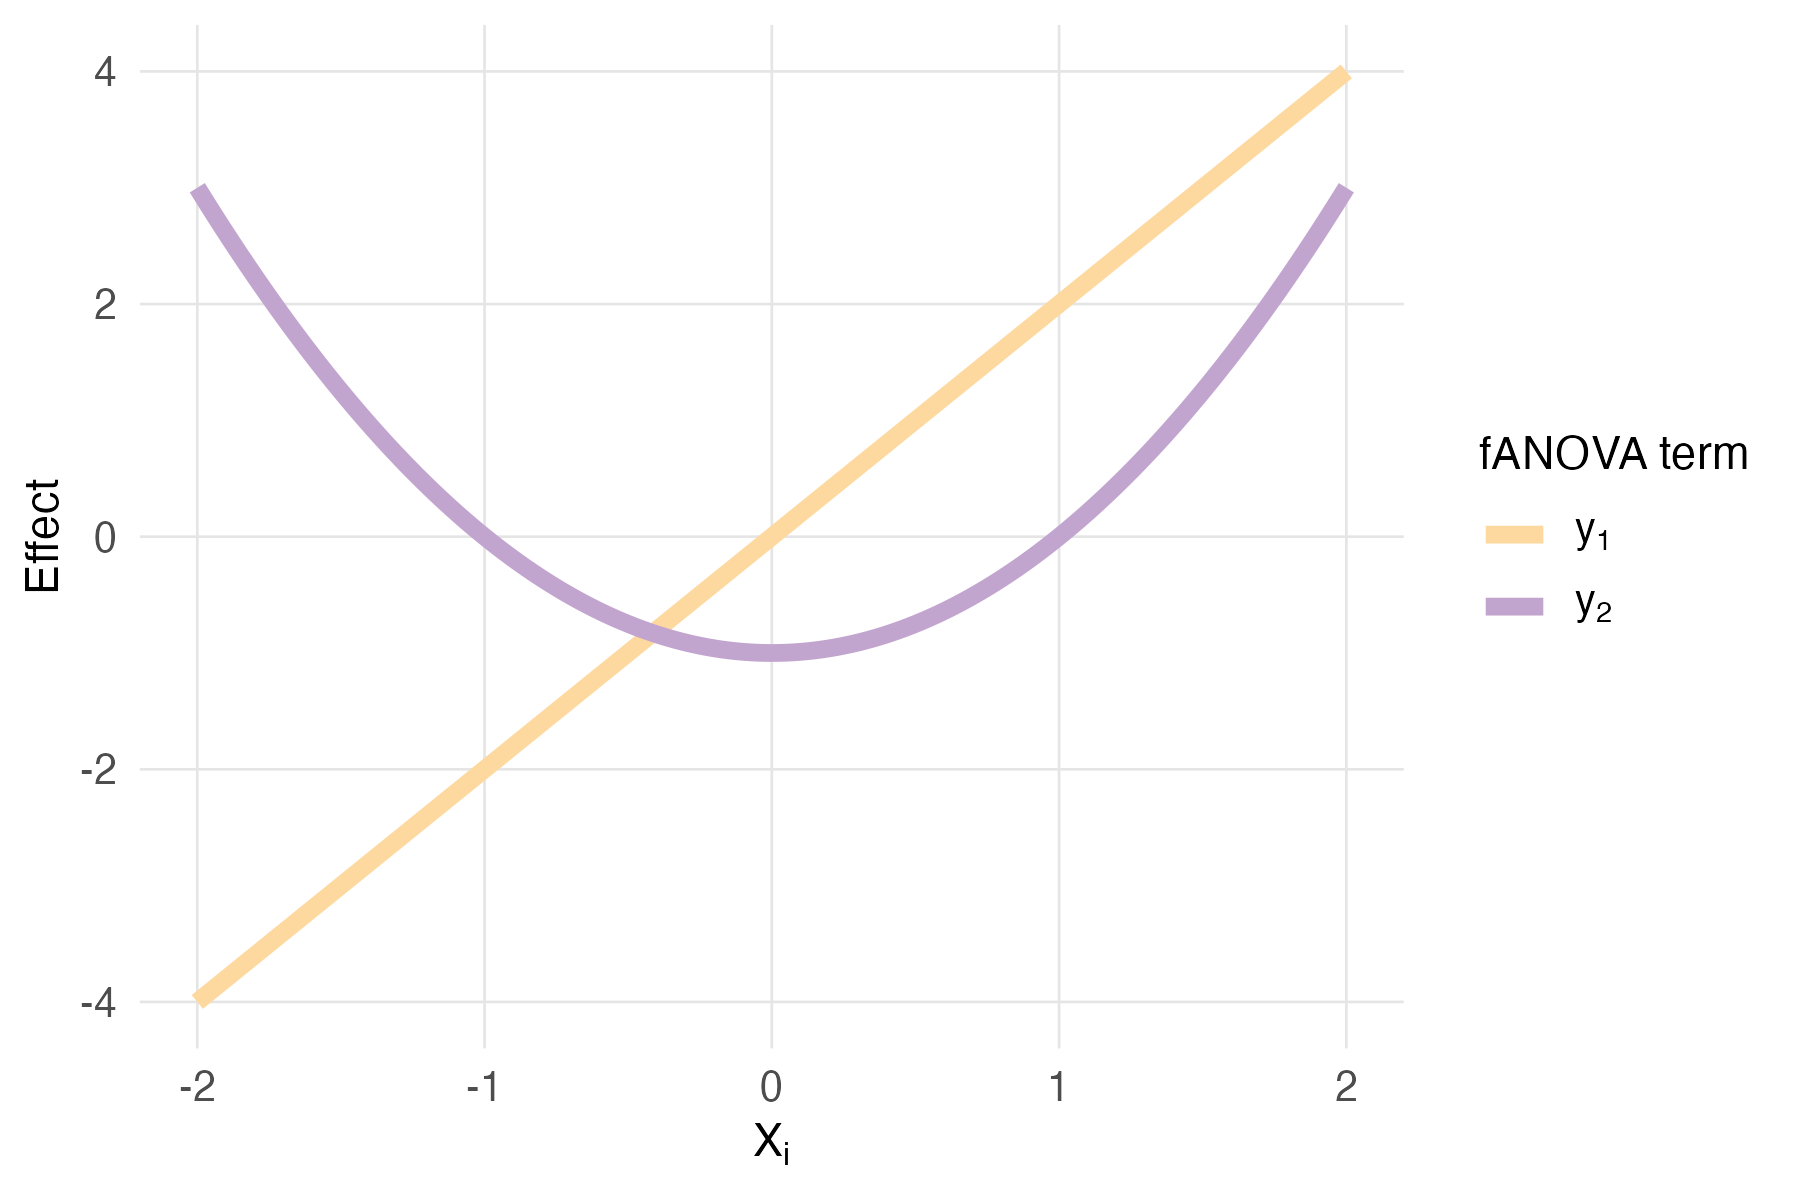
\includegraphics[width=\linewidth]{../images/experiment_section/classical_ex_1_a1p20_a2p00_a11p00_a22p10_a12p10_rhop00_main.png}
    \column{0.5\textwidth}
      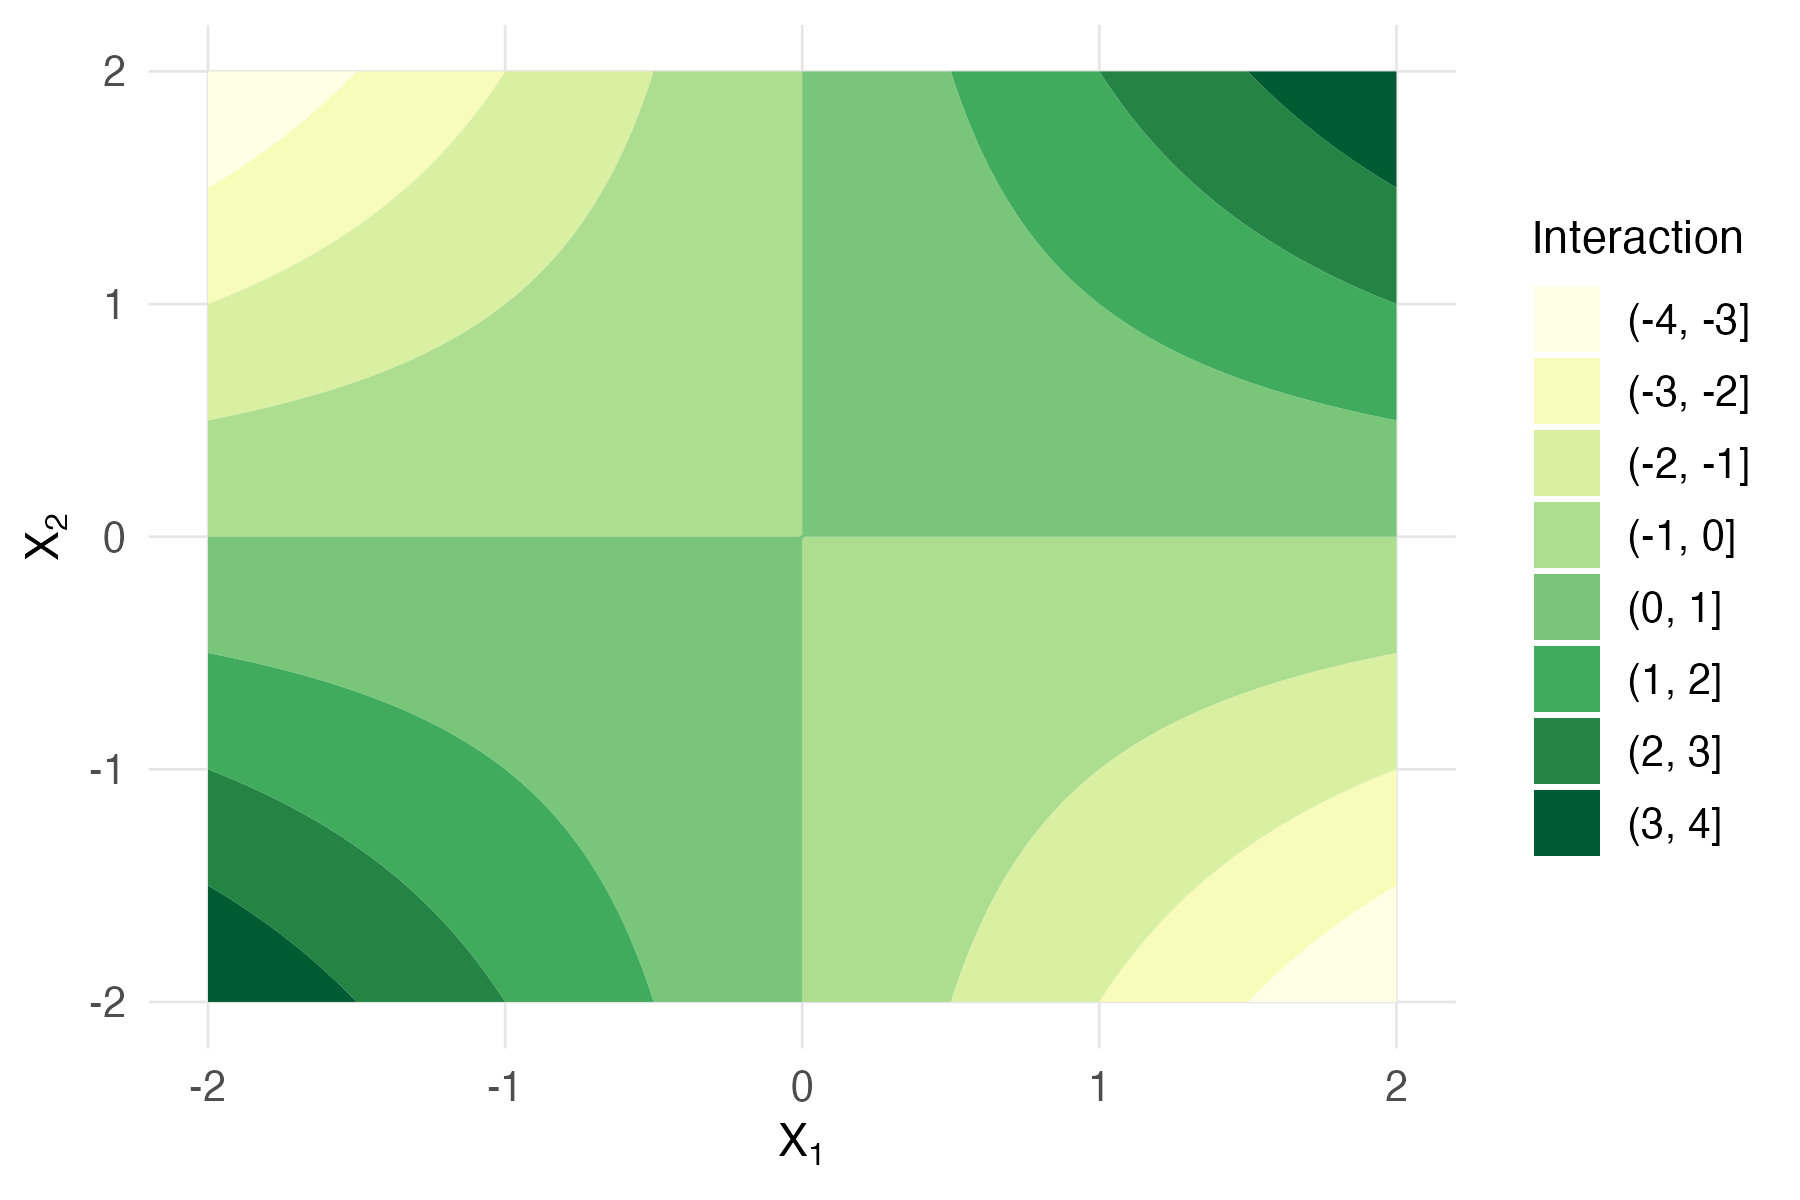
\includegraphics[width=\linewidth]{../images/experiment_section/classical_ex_1_a1p20_a2p00_a11p00_a22p10_a12p10_rhop00_interaction.png}
  \end{columns}
\end{frame}

% fANOVA through lens of Orthogonal Projections
\begin{frame}{Reminder: Definition of Orthogonal Projection} % How do we define it?
  \begin{align*}
    \Pi_{\mathcal{G}}y = \arg\min_{g \in \mathcal{G}} \|y - g\|^2
= \arg\min_{g \in \mathcal{G}} \mathbb{E}[(y(\boldsymbol{X}) - g(\boldsymbol{X}))^2].
\end{align*}
  \begin{itemize}
    \item $\mathcal{G}$ : linear subspace of $\mathcal{L}^2$ we project onto
    \item $g$ all functions in the subspace
  \end{itemize}
\end{frame}

\begin{frame}{fANOVA as Orthogonal Projection} % How does it relate to orthogonal projection?
\begin{align*}
    y_{\emptyset}
    &= \mathbb{E}[y(\boldsymbol{X})] \\ 
    &= \arg \min_{a \in \mathbb{R}} \mathbb{E}[(y(\boldsymbol{X}) - a)^2] \\ 
    &= \arg \min_{g_0 \in \mathcal{G}_0} \|y - g_0\|^2
    = \Pi_{\mathcal{G}_0}y,
\end{align*}
\begin{align*}
    y_u(.) 
    &= \mathbb{E}[y(\boldsymbol{X}) \mid X_{u} = .] - \sum_{v \subsetneq u} y_v(.) \\ 
    &= \arg \min_{g_u \in \mathcal{G}_u} \mathbb{E}[(y(\boldsymbol{X}) - g_u(.))^2] - \sum_{v \subsetneq u} y_v(.) \\ 
    &= (\Pi_{\mathcal{G}_u}y)(.) - \sum_{v \subsetneq u} y_v(.)
\end{align*}

  
\end{frame}


\begin{frame}{Equality to Hoeffding Decomposition} % How does it relate to Hoeffding?
  \begin{block}{Hoeffding Decomposition}
    \begin{align}
    y(\boldsymbol{X})
=
\sum_{A \subseteq D} 
y_A(\boldsymbol{X}_A),
\qquad
D := \{1,\dots,N\},
\end{align}
where, for each $A \subseteq D$, the component function $y_A$ is defined by:
\begin{align}\label{eq:hoeffding_components}
    y_A(\boldsymbol{X}_A)
=
\sum_{B \subseteq A}
(-1)^{|A|-|B|}
\,\mathbb{E}\!\left[
  y(\boldsymbol{X}) 
  \,\middle|\, 
  \boldsymbol{X}_B
\right],
\end{align}
  where $y_u$ are orthogonal components.
  \end{block}
  \begin{itemize}
    \item Classical fANOVA and Hoeffding decomposition yield same components under zero-centered inputs
    \item Both assume independence of input variables
  \end{itemize}
  
\end{frame}

\begin{frame}{Hoeffding Decomposition Example} % Example of Hoeffding decomposition
  \begin{align*}
    y(x_1, x_2) = 2x_1 + x_2^{2} + x_1 x_2
  \end{align*}
  \begin{align*}
    % --- constant component
    y_{\emptyset}
    &= \mathbb{E}[y(X_1,X_2)] 
     = 2\,\mathbb{E}[X_1] + \mathbb{E}[X_2^2] + \mathbb{E}[X_1 X_2] 
     = 1,
    \\[1.2em]
    % --- first-order component for X1
    y_{\{1\}}(x_1)
    &= \sum_{B \subseteq \{1\}} (-1)^{1-|B|}
       \,\mathbb{E}[y(\boldsymbol{X})\,|\,X_B] \\[2pt]
    &= -\,\mathbb{E}[y] + \mathbb{E}[y|X_1=x_1] \\[2pt]
    &= -1 + (2x_1 + \mathbb{E}[X_2^2] + x_1\mathbb{E}[X_2]) \\[2pt]
    &= 2x_1,
    \\[1.2em]
    % --- first-order component for X2
    y_{\{2\}}(x_2)
    &= \sum_{B \subseteq \{2\}} (-1)^{1-|B|}
       \,\mathbb{E}[y(\boldsymbol{X})\,|\,X_B] \\[2pt]
    &= -\,\mathbb{E}[y] + \mathbb{E}[y|X_2=x_2] \\[2pt]
    &= -1 + (2\mathbb{E}[X_1] + x_2^2 + x_2\mathbb{E}[X_1]) \\[2pt]
    &= x_2^2 - 1.
\end{align*}
\end{frame}

\begin{frame}
  \begin{align*}
    % --- second-order interaction component
    y_{\{1,2\}}(x_1,x_2)
    &= \sum_{B \subseteq \{1,2\}} (-1)^{2-|B|}
       \,\mathbb{E}[y(\boldsymbol{X})\,|\,X_B] \\[2pt]
    &= (+1)\,\mathbb{E}[y] 
     - \mathbb{E}[y|X_1=x_1]
     - \mathbb{E}[y|X_2=x_2]
     + y(x_1,x_2) \\[2pt]
    &= 1 - (2x_1+1) - (x_2^2) + (2x_1+x_2^2+x_1x_2) \\[2pt]
    &= x_1 x_2.
\end{align*}

\[
y(x_1,x_2)
= y_{\emptyset} + y_{\{1\}}(x_1) + y_{\{2\}}(x_2) + y_{\{1,2\}}(x_1,x_2)
= 1 + 2x_1 + (x_2^2 - 1) + x_1 x_2
\]

\end{frame}




\section{Generalized fANOVA}
\begin{frame}{Example with Dependent Inputs ($\rho = 0.8$)} % How does it look?
  \begin{columns}
    \column{0.5\textwidth}
      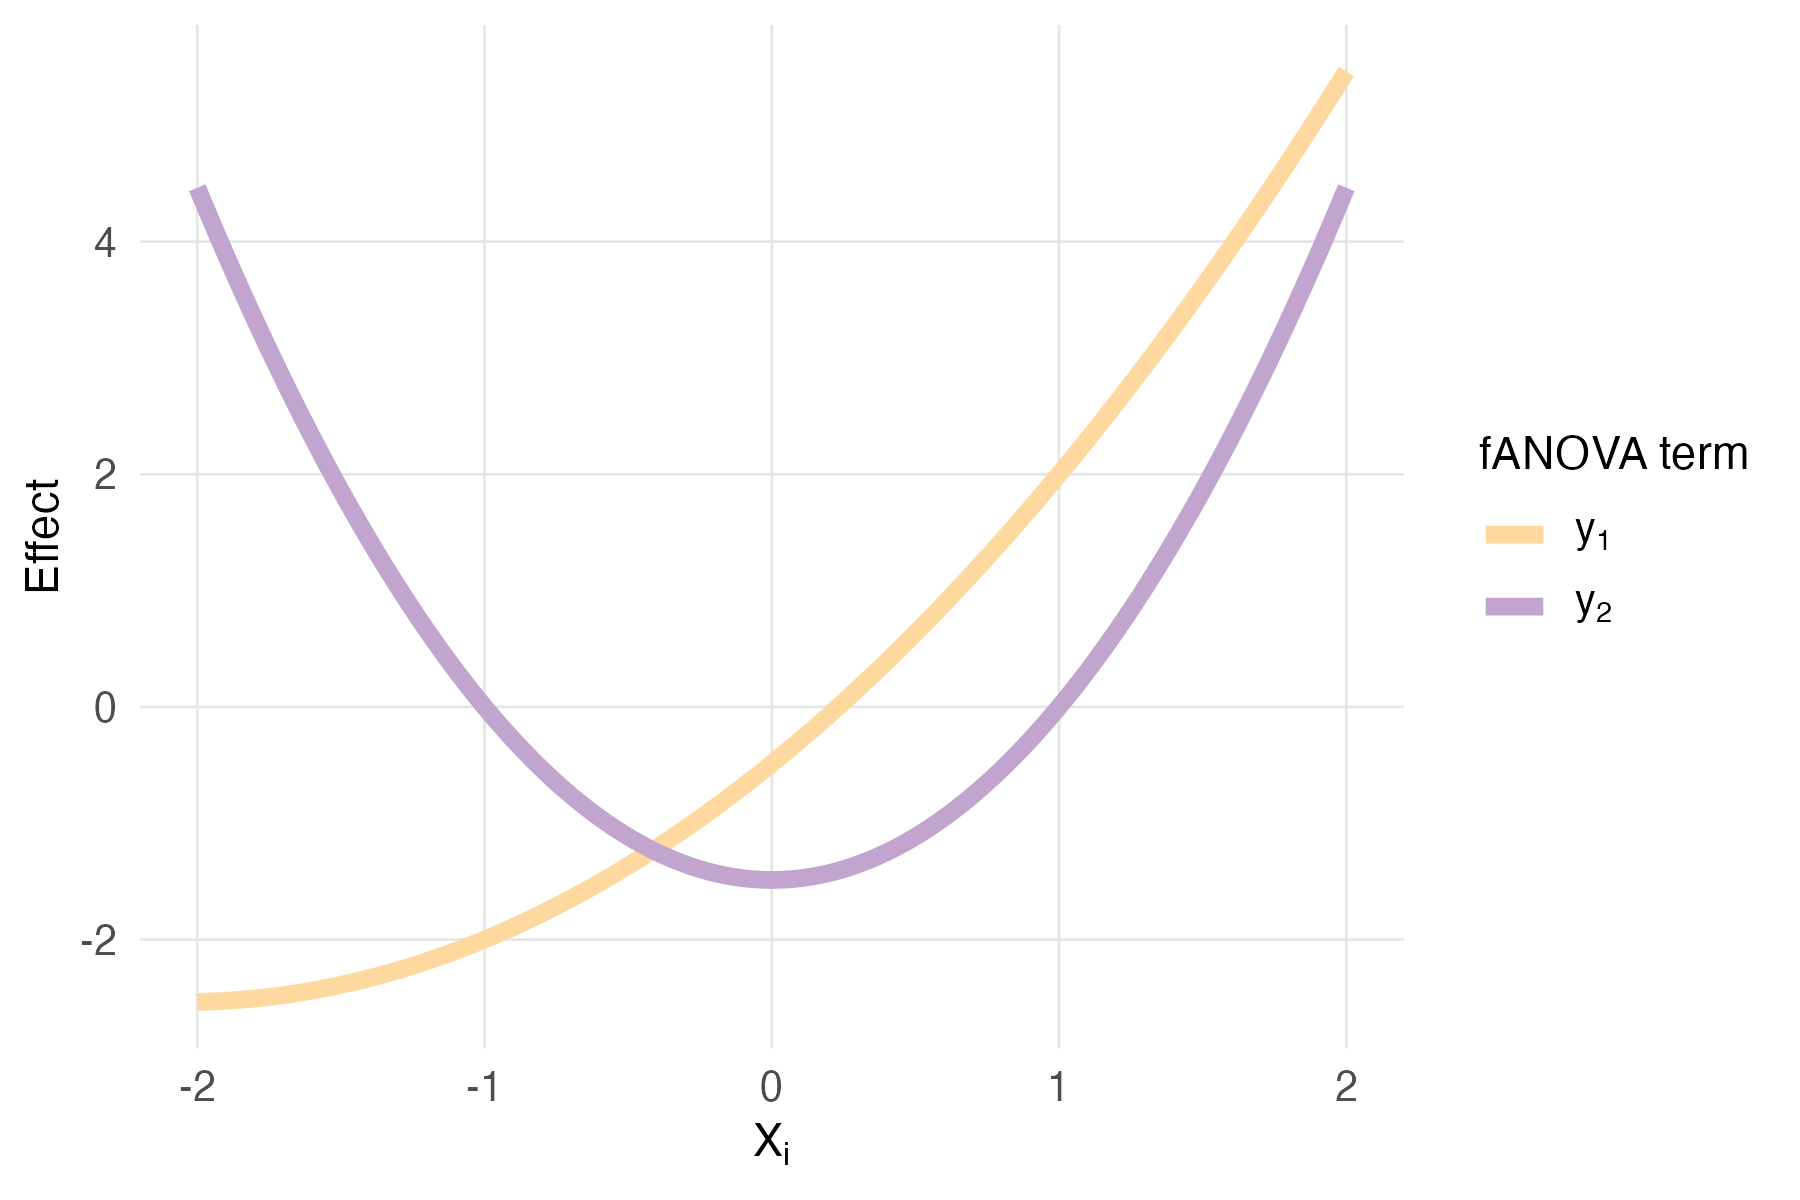
\includegraphics[width=\linewidth]{../images/experiment_section/gen_ex_1_a1p20_a2p00_a11p00_a22p10_a12p10_rhop08_main.png}
    \column{0.5\textwidth}
      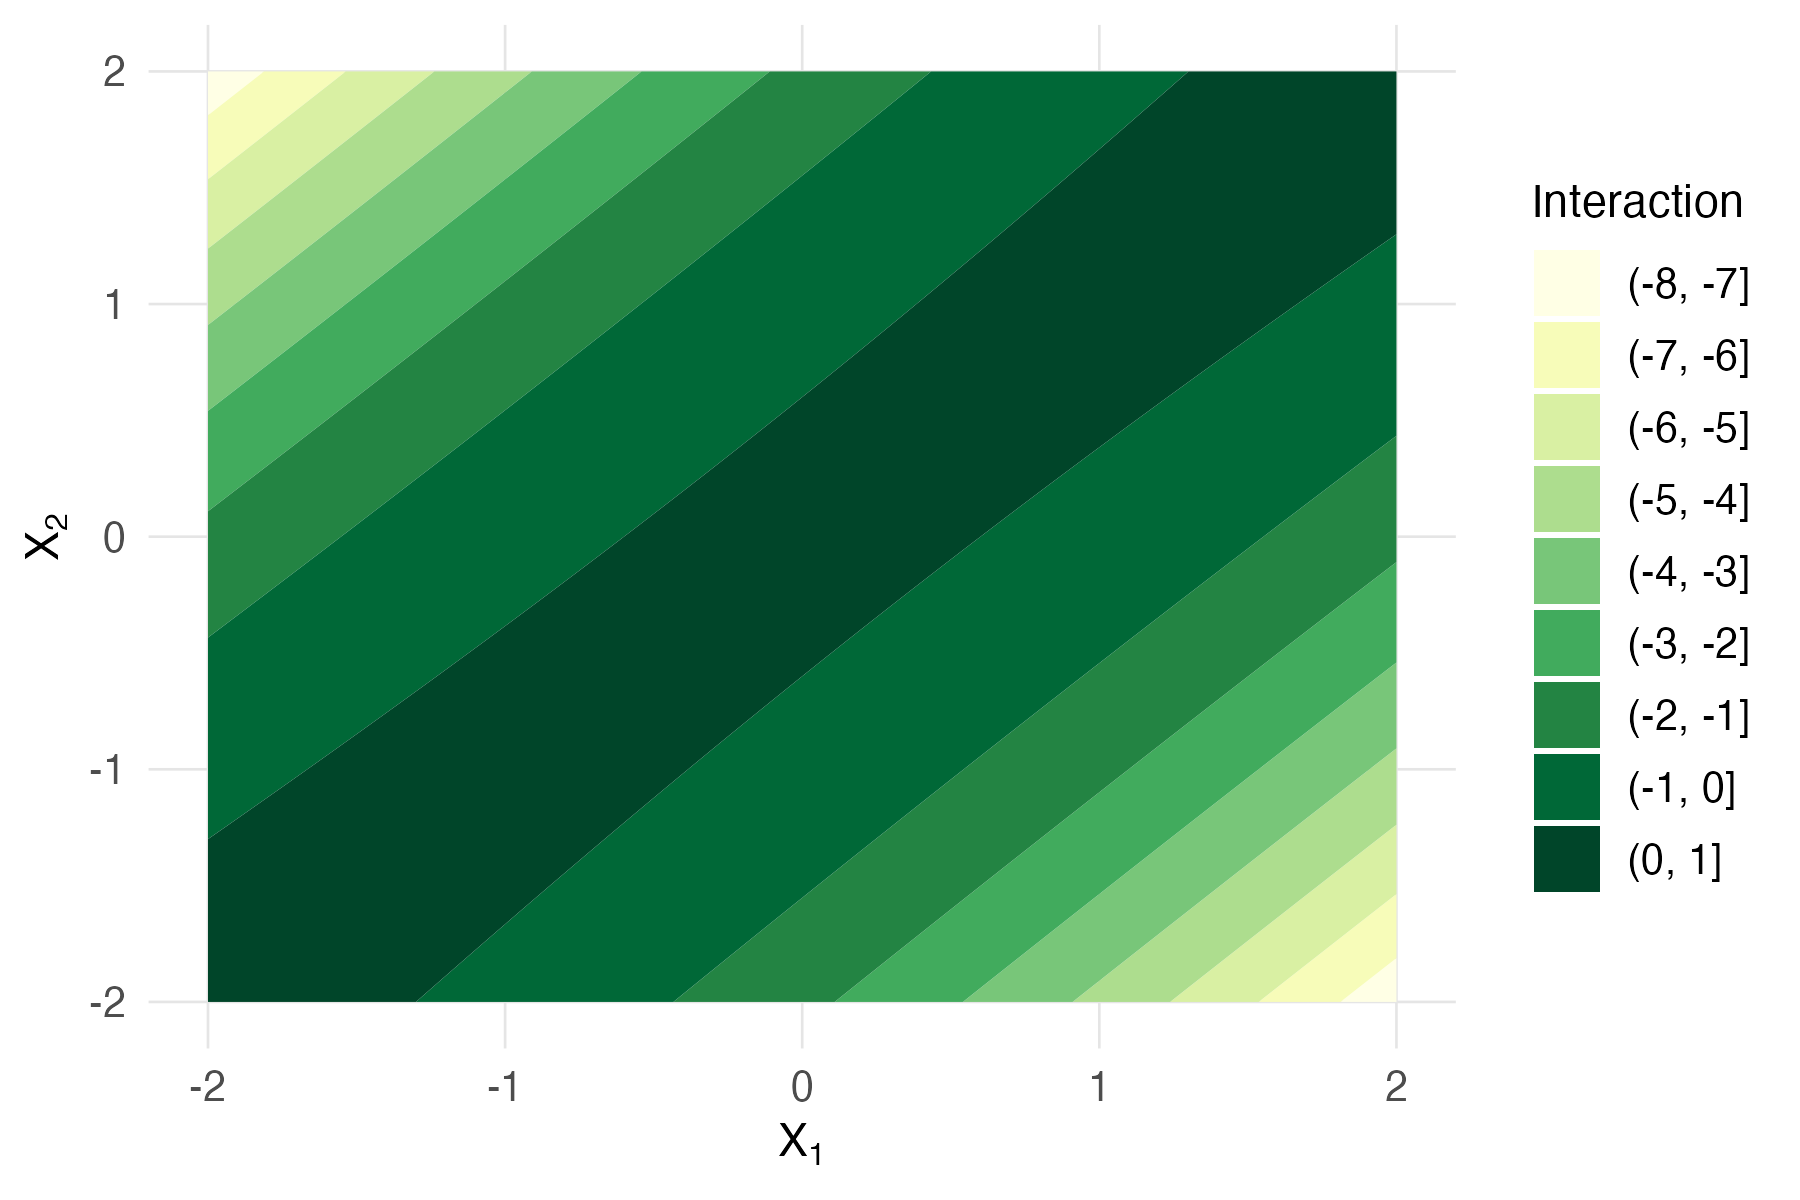
\includegraphics[width=\linewidth]{../images/experiment_section/gen_ex_1_a1p20_a2p00_a11p00_a22p10_a12p10_rhop08_interaction.png}
  \end{columns}
\end{frame}

%==================================================
% Slide 2 – Conditions (Weaker Annihilating Conditions)
%==================================================
\begin{frame}{Weaker Annihilating Conditions}
  \begin{block}{Weak Annihilating Conditions}
    \[
      \int_{\mathbb{R}} y_{u, G}(\boldsymbol{x}_u) f_{\boldsymbol{X}_u}(\boldsymbol{x}_u) d\nu (x_i) = 0 \quad \text{for} \quad i \in u \neq \emptyset.
    \]
  \end{block}
  \begin{itemize}
    \item Allows dependent input distributions
    \item Leads to hierarchical orthogonality
  \end{itemize}
\end{frame}

%==================================================
% Slide 3 – Properties
%==================================================
\begin{frame}{Key Properties (Generalized)}
  \[
  \mathbb{E}[y_{u, G}(\boldsymbol{X}_u)] := \int_{\mathbb{R}^N} y_{u, G}(\boldsymbol{x}_u) f_{\boldsymbol{X}}(\boldsymbol{x}) \, d\nu (\boldsymbol{x}) = 0.
  \]
  \[
  \mathbb{E}[y_{u, G}(\boldsymbol{X}_u)y_{v, G}(\boldsymbol{X}_v)] := \int_{\mathbb{R}^N} y_{u, G}(\boldsymbol{x}_u) y_{v, G}(\boldsymbol{x}_v) f_{\boldsymbol{X}}(\boldsymbol{x}) \, d\nu (\boldsymbol{x}) = 0.
  \]
  \begin{itemize}
    \item Zero mean components remain
    \item Orthogonality is weaker: hierarchical
  \end{itemize}
\end{frame}

%==================================================
% Slide 4 – Construction
%==================================================
\begin{frame}{Component Definition (Coupled System)}
  \begin{align}
    y_{\emptyset,G} &= \int_{\mathbb{R}^N} y(\boldsymbol{x}) f_{\boldsymbol{X}}(\boldsymbol{x}) \, d \nu(\boldsymbol{x}) \\[3ex]
    y_{u,G}(\boldsymbol{X}_u) &= \int_{\mathbb{R}^{N - |u|}} y(\boldsymbol{X}_u, \boldsymbol{x}_{-u}) f_{-u}(\boldsymbol{x}_{-u}) \, d \nu(\boldsymbol{x}_{-u}) - \sum_{v \subsetneq u} y_{v,G}(\boldsymbol{X}_v) \notag \\
    &\quad - \sum_{\substack{\emptyset \ne v \subseteq \{1,\dots,N\} \\ v \cap u \ne \emptyset,\ v \not\subset u}} \int_{\mathbb{R}^{|v \cap -u|}} y_{v,G}(\boldsymbol{X}_{v \cap u}, \boldsymbol{x}_{v \cap -u}) f_{v \cap -u}(\boldsymbol{x}_{v \cap -u}) \, d \nu(\boldsymbol{x}_{v \cap -u}).
\end{align}
  \begin{itemize}
    \item All components solved simultaneously
    \item Depends on marginal densities and coupling terms
  \end{itemize}
\end{frame}

%==================================================
% Slide 5 – Link Back to Example
%==================================================
\begin{frame}{How to Construct the Components}
    \begin{itemize}
        \item Coupled system $\rightarrow$ difficult to obtain analytical solutions
        \item Use alternative method via Fourier Polynomial (\cite{rahman2014})
        \item Building blocks: mutually orthogonal, zero-mean basis functions $\psi_{i, j}$, coefficients $c_{i, j}$
    \end{itemize}
\end{frame}

\begin{frame}{Basis Representation of a Polynomial}
    \begin{align*}
y(x_1,x_2) 
&= a_0 + a_1 x_1 + a_2 x_2 
   + a_{11} x_1^2 + a_{22} x_2^2 + a_{12} x_1 x_2 \\[0.5em]
&= c_0 
   + c_{1,1}\,\psi_{1,1}(x_1) 
   + c_{2,1}\,\psi_{2,1}(x_2) \\[0.5em]
&\quad
   + c_{1,2}\,\psi_{1,2}(x_1)
   + c_{2,2}\,\psi_{2,2}(x_2)
   + c_{12,11}\,\psi_{12,11}(x_1,x_2) \\[0.5em]
&= 
   \underbrace{c_0}_{y_0}
   + \underbrace{\big(c_{1,1}\,\psi_{1,1}(x_1) 
                     + c_{1,2}\,\psi_{1,2}(x_1)\big)}_{y_1(x_1)} \\[0.5em]
&\quad
   + \underbrace{\big(c_{2,1}\,\psi_{2,1}(x_2) 
                     + c_{2,2}\,\psi_{2,2}(x_2)\big)}_{y_2(x_2)} \\[0.5em]
&\quad
   + \underbrace{c_{12,11}\,\psi_{12,11}(x_1,x_2)}_{y_{12}(x_1,x_2)}.
\end{align*}
\end{frame}

\begin{frame}{Basis Functions proposed by Rahman (2014)\cite{rahman2014}}
    \begin{align*}
\psi_{\emptyset}(x_1,x_2) &= 1, \\[0.5em]
\psi_{1,1}(x_1) &= x_1, \\[0.5em]
\psi_{2,1}(x_2) &= x_2, \\[0.5em]
\psi_{1,2}(x_1) &= x_1^2 - 1, \\[0.5em]
\psi_{2,2}(x_2) &= x_2^2 - 1, \\[0.5em]
\psi_{12,11}(x_1,x_2) &= \frac{\rho (x_1^2 + x_2^2)}{1 + \rho^2} 
                         - x_1 x_2 
                         + \frac{\rho(\rho^2 - 1)}{1 + \rho^2},
\end{align*}
\end{frame}

\begin{frame}{Alternative Generalization of fANOVA, \cite{hooker2007}}
    \begin{align*}
\left\{ y_{u, G}(\boldsymbol{x}_u) \,\middle|\, u \subseteq d \right\}
= \arg\min_{\{g_u \in \mathcal{L}^2(\mathbb{R}^{|u|})\}} 
\int_{\mathbb{R}^N} \left( \sum_{u \subseteq d} g_u(\boldsymbol{x}_u) - y(\boldsymbol{x}) \right)^2 
f_{\boldsymbol{X}}(\boldsymbol{x}) \, d \nu (\boldsymbol{x}),
\label{eq:generalized_fanova_components_hooker}
\end{align*}
subject to hierarchical orthogonality conditions:
\begin{align*}
    \forall v \subseteq u,\ \forall g_v:\ 
    \int_{\mathbb{R}^N} y_u(\boldsymbol{x}_u) g_v(\boldsymbol{x}_v) 
    f_{\boldsymbol{X}}(\boldsymbol{x}) \, d \nu (\boldsymbol{x}) = 0.
\end{align*}
\end{frame}

\begin{frame}{Variance Decomposition, \cite{sobol1993sensitivity}}
    \[
    \mu := \mathbb{E}[y(\boldsymbol{X})] = y_{\emptyset,G}.
    \]
    \begin{align*}
\sigma^2 
&:= \mathbb{E}\left[ \left( y(\boldsymbol{X}) - \mu_G \right)^2 \right] \notag \\
&= \mathbb{E} \left[ \left( y_{\emptyset,G} + \sum_{u} y_{u,G}(\boldsymbol{X}_u) - y_{\emptyset,G} \right)^2 \right] \notag \\
&= \mathbb{E} \left[ \left( \sum_{u} y_{u,G}(\boldsymbol{X}_u) \right)^2 \right] \notag \\
&= \sum_{u} \mathbb{E} \left[ y_{u,G}^2(\boldsymbol{X}_u) \right]
+ \sum_{\substack{u \not\subseteq v,\, v \not\subseteq u}} 
\mathbb{E} \left[ y_{u,G}(\boldsymbol{X}_u) y_{v,G}(\boldsymbol{X}_v) \right],
\end{align*}
    
\end{frame}


\section{Conclusion}
% Recaps of what I did
% 1. gave historical context of fANOVA by showing origins of the method and how it evolved over time
% We started by working through the historical context of the fANOVA decomposition. We explored the origins of the fANOVA method rooted in mathematical work by \cite{hoeffding1948} and \cite{sobol1993sensitivity}. We saw how the method was picked up by following researchers in different contexts.

% 2. formal introduction, to classical fANOVA
% synthesise multiple sources into one clean, general but not 
% too general formulation of the method
% looked at key properties that characterize fANOVA + distinguish it from other IML methods

% --->> could work out a bit more (for now mostly conceptually)
% uniqueness of fANOVA in comparison to other methods
% e.g. say that it is a global technique, decomposes the function
% it is model agnostic, global etc.

% 3. generalization of fANOVA
% we saw how classical fANOVA breaks down under dependent inputs
% weak independence might not be problem but if features are strongly correlated fANOVA will yield misleading results
% the generalization is in the end doing nothing other than letting go of the product type probability measure 
% but constructing components that still satisfy the nice properties and add up to the original function is not trivial 
% there are multiple ways to generalize the components, we mostly
% focused on work by Hooker and Rahman


% we unified different formulations of the method using the parallel
% between conditional expected value and orthogonal projections
% this is the key to bringing different formulations together and also generlizing the idea of fANOVA
% to different scenarios

% approximation of fANOVA done via sampling, lagrange multiplier etc.

The fANOVA decomposition is a foundation method that has been studied from many perspectives, with recent interest driven by its potential in model interpretability. Its key strength lies in producing terms that represent the unique contribution of each variable or interaction, cleanly separated from one another without mixing effects.\par

Despite being established in the literature, we found a lack of unified formalization and notational clarity in the literature, which we aimed to address in this work.\par

We began by revisiting the classical fANOVA decomposition, bridging Sobols initial formulation with more recent developments. We filled small gaps in mathematical proofs and established a direct connection to conditional expectations and orthogonal projections, which we argue is key to unifying different existing notations and formal approaches. Alongside the functional decomposition, we presented the variance decomposition, which underpins Sobol indices and links the fANOVA structure to sensitivity analysis.\par

Next, we extended the decomposition to dependent input variables. Here, multiple approaches exist; we focused on the frameworks of \cite{hooker2007} and \cite{rahman2014}. Using an illustrative example, we encountered the close relation between the fANOVA and Hoeffding decompositions and demonstrated that obtaining interpretable fANOVA components under dependence requires careful constraint selection. We also noted that closed-form solutions for the generalized components are difficult to obtain in practice and remain an open problem. Nevertheless, the associated variance decomposition still holds, allowing for the construction of generalized Sobol indices.\par

To complement the theoretical work, we visualized fANOVA components for simple polynomial functions with Gaussian inputs. These visualizations illustrated how fANOVA separates effects, but were limited to simple functions and Gaussian inputs.\par

This work did not present a full numerical treatment of Sobol indices, only touching on variance decomposition as their foundation. Our empirical demonstrations were restricted to toy problems; applying fANOVA in practice will require estimation methods suitable for trained models on real data. We also briefly mentioned the ability of fANOVA to purify interaction effects \citep{lengerich2020} and its relation to other interpretability techniques (e.g., PD, Shapley values \citep{fumagalli2025}) but did not explore these connections in depth.\par

Future work could extend Rahman’s polynomial expansion approach to more complex polynomials and non-Gaussian input distributions, and further investigate mathematical connections to other interpretability frameworks.
Additionally, a lack of publicly available software for performing fANOVA remains a barrier to its widespread adoption, so developing robust, open-source implementations would be an important step toward enabling its use in practical model interpretability.

% Recap: fANOVA is a foundation method studied from many perspectives; most recently researchers caught interest in fANOVA for its potential in model interpretability - what makes it special is that the fANOVA terms represent the unique contribution of each variable or interaction - they are cleanly separated from each other and do not mix up.
% Though so widely used we found a lack of unified formalization and notational clarity, which we hope to have provided with this work.\par
% We started with the classical fANOVA decomposition; well-known in literature \cite{rahman2014} but we filled some small gaps in mathematical proofs, and wrote out the paralel to conditional expected value and orthogonal projections, which is the key to unifying different notations and approaches to the formalization of fANOVA.
% We briefly adressed the variance decomposition, which goes hand in hand with the functional decomposition and is the foundation of Sobol indices.\par
% We then generalized the fANOVA decomposition to dependent inputs. Here different approaches exist, and we focused on the work by \cite{hooker2007} and \cite{rahman2014}. Based on an example we saw that the fANOVA decomposition is closely related to Hoeffding decomposition and to obtain the real fANOVA components under independence with their clear interpretation it is necessary to construct a careful set of constraints.
% Obtaining a closed form solution for the generalized components is challenging in most cases and remains an open problem. Though more complex the variance decomposition still works in principle and allows for the construction of generalized Sobol indices.\par
% Lastly, we experimented with visualizing the fANOVA components of different functions, while we stayed within the realm of two degree polynomials with Gaussian inputs.\par
% % Limitations of this work:
% % did not really present Sobol indices, only mentioned the variance decomposition
% % Illustrated fANOVA with toy example in really limited setting; would be intersting to train a model on real data and really apply fANOVA decomposition; for this however we need an estimation approach
% % In the final section it was elluded briefly: fANOVA and how it can purify interactions, did not go into depth but this is an interesting topic highly relevant to fANOVA and interpretability
% % Briefly contrasted fANOVA to other IML methods here and there but did not formally compare to other methods; would be very interesting to examine this from a mathematical pespective: direct connection to partial dependence and recent work also shows mathematical connection to Shapley values \cite{fumagalli2025}.
% For future work it would be interesting to study the extension of Rahman's polynomial expansion approach for other distribution assumptions and more complex polynomials. Moreover, as we argued in the end, there is a lack of software implementations for fANOVA decomposition, which is a barrier to its application in model interpretability.


% fANOVA powerful theory, sound mathematical foundation, but without standardized software implementation application to IML difficult.
% Parallels to Shapley values, unified under a game theoretic approach; \cite{fumagalli2025} recently established this parallel, would be very interesting to investigate further.
% Use Rahmans methods and extend it to different distribution assumptions.



\section{Extra Slides}
% Show important proofs
% show the foundational sätze they use

\begin{frame}{Classical fANOVA Proofs}
    \begin{itemize}
        \item Zero mean property: factorized density, Fubinis Theorem, strong annihilating conditions
        \item Mutual orthogonality: factorized density, Fubinis Theorem, strong annihilating conditions
    \end{itemize}
\end{frame}

\begin{frame}{Generalized fANOVA Proofs}
    \begin{itemize}
        \item Zero mean property: separating $x$ into subvectors, marginal density, Fubinis Theorem, weak annihilating conditions
        \item Hierarchical orthogonality: set the scene, u is a proper subset of v $u \subsetneq v$, so there is an index in u which is not in v; divide $x_u$ into subvectors, marginal density, Fubini and weak annihilating conditions
        \item Weak annihilating becomes strong under independence: assume the weak ones, product density, factor out
        \item Three integration cases: distinguish between different relationships u and v, depending on the relationship the integral w.r.t. to marginal density simplifies
        \item Generalized fANOVA components by Rahman: first build constant term; for nonconstant terms use integration cases
        \item Integration constraint Hooker: show that hierarchical orthogonality is fulfilled if the conditions hold, show that it is not fulfilled if they do not hold; but why exactly these conditions a bit unclear
        \item Take a look at Sobols proof again
    \end{itemize}
\end{frame}

\begin{frame}{Relevant External Links}
    \begin{itemize}
        \item \url{https://docs.google.com/spreadsheets/d/1K5ECL6hDPDnHwM_k342xa29H-vHWzdk27PTgDHUwfFE/edit?usp=sharing} - Table with fANOVA-related literature
    \end{itemize}
\end{frame}

\begin{frame}[allowframebreaks]
        \frametitle{References}
        \bibliographystyle{plain}
        \bibliography{../bibliography_2, ../bibliography_manual}
\end{frame}

\end{document}


